\documentclass{kit}

\usepackage[ruled,vlined]{algorithm2e}
\SetAlgorithmName{}{}
% \SetAlgoCaptionSeparator{}

\author{Julius Vater - 2603322}
\title{Digitaltechnik und Entwurfsverfahren Zusammenfassung}
\begin{document}
\maketitle
\tableofcontents
\pagebreak
\section{Zahlensysteme}
  \subsection{Umrechnungen in Zahlensysteme}
    \begin{itemize}
      \item Von Basis $b$ zu Basis 10:
          $$(\lambda_n...\lambda_0)_b=\sum_{i=0}^n\lambda_i*b^i=z_{10}$$
      \item Von Basis 10 zu Basis $b$
            \begin{algorithm}
              \caption{Euklidischer Algorithmus}
              find i $\in\nat:b^{i+1}>$ val $\ge b^i$\;
              \While{i $\ge0$}
              {
                $z_i:=$ val div $b^i$\;
                val := val mod $b^i$\;
                $i=i-1$\;
              }
              \Return z;
            \end{algorithm}
            \begin{algorithm}
              \caption{Horner-Shema}
              $i:=0$\;
              \While{val $\neq0$}
              {
                $z_i:=$ val mod $b$\;
                val := val div $b$\;
                $i=i-1$\;
              }
              \Return z;
            \end{algorithm}
    \end{itemize}
  \newpage
  \subsection{Kodierung von ganzen Zahlen}
    \subsubsection{Vorzeichenbit}
      \begin{itemize}
        \item Erstes Bit Vorzeichen ($-:=1,+:=0$)
        \item Weitere Bits stellen die Zahl dar
        \item Problmeme:
          \begin{itemize}
            \item Redundante Nullen: $0$ und $-0$ verschiedene Codes
            \item Addition: $-1+4=1001\oplus0100=1101=-5$
          \end{itemize}
      \end{itemize}
    \subsubsection{Einerkomplement}
      \begin{itemize}
        \item Positive Zaheln werden einfach so dargestellt
        \item Negative Zaheln entstehen durch bitweise invertieren. Dadurch folgt ein implizites 
          Vorzeichen
        \item Problem: Addition beim überschreiten der 0 ist fehlerhaft und nicht ohne Sonderregel
          durchführbar
          \begin{itemize}
            \item $-1=\lnot00000001=11111110$
            \item $2=00000010$
            \item $2+(-1)=00000010+11111110=00000000$
          \end{itemize}
      \end{itemize}
    \subsubsection{Zweierkomplement}
      \begin{itemize}
        \item Positive Zaheln werden einfach so dargestellt
        \item Negative Zaheln entstehen durch bitweise invertieren und Addition um eins 
          $(\lnot(z)+1)$. Dadurch folt ein implizites Vorzeichenbit
        \item Dadurch entsteht keine Redundanz und Addition ist einfach möglich
      \end{itemize}
    \subsubsection{Offset-Dual-Darstellung}
      \begin{itemize}
        \item Zweierkomplement-Darstellung mit einem Offset
        \item offset = $2^{n-1}$ (i.d.R. damit die kleinste (negative) Zahl den Code 0 hat)
        \item ZK(z)+offset = $(\lnot z)$ + 1 + offset
        \item Vorzug: Lexigraphisch vergleichbar
      \end{itemize}
    \subsubsection{IEEE-754-Standart}
      \begin{itemize}
        \item $x=s*1,m*b^{c-\text{Bias}}$\\
          s: Vorzeichen, m: Mantisse, b: Basis, c: Characteristik\\\\
          \begin{tabular}{|c|c|c|c|c|}
            \hline
            Name & $\sum$-Bits & Characteristik & Mantisse & Bias \\
            \hline 
            \hline
            single & 32 Bits & 8 Bits & 23 Bits & 127 \\
            \hline
            double & 64 Bits & 11 Bits & 52 Bits & 1023\\
            \hline
          \end{tabular}
      \end{itemize}
    \subsubsection{BCD}
      \begin{itemize}
        \item Tetraden, also immer vier Bits definieren eine Dezimalzahl
        \item Mit vier Bits sind die Zahlen von null bis fünfzehn darstellbar, so folgen sechs 
          Pseudotetraden\\\\
          \begin{tabular}{|c|c||c|c||c|c||c|c|}
            \hline
            0 & 0000 & 4 & 0100 & 8 & 1000 & X & 1100\\
            1 & 0001 & 5 & 0101 & 9 & 1001 & X & 1101\\
            2 & 0010 & 6 & 0110 & X & 1010 & X & 1110\\
            3 & 0011 & 7 & 0111 & X & 1011 & X & 1111\\
            \hline
          \end{tabular}
      \end{itemize}
    \subsubsection{Gray Kodierung}
      \begin{itemize}
        \item Zwischen zwei benachbarten Zahlen ändert sich immer nur ein bit\\\\
          \begin{tabular}{|c|c||c|c||c|c||c|c|}
            \hline
            0 & 0000 & 4 & 0110 & 8 & 1100 & X & 1010\\
            1 & 0001 & 5 & 0111 & 9 & 1101 & X & 1011\\
            2 & 0011 & 6 & 0101 & X & 1111 & X & 1001\\
            3 & 0010 & 7 & 0100 & X & 1110 & X & 1000\\
            \hline
          \end{tabular}
      \end{itemize}
  \subsection{Fehlerkorrigierende Codes}
    \subsubsection{Quersumme von Binärzahlen}
      \begin{itemize}
        \item $QS(b_n,...,b_0)=b_n\oplus\cdots\oplus b_0$
        \item Wenn sich ein Bit ändert, ändert sich die Quersumme
      \end{itemize}
    \subsubsection{Paritätsbits}
      \begin{itemize}
        \item Einem Binärwort wird um das Quersummenbit ergänzt.\\
          \phantom{Hallo}$b_n,\dots,b_0\Rightarrow b_n,\dots,b_0,QS(b_n,\dots,b_0)$
        \item Erkennen von Fehlern ungerader Anzahl (liegen Fehler gerader Anzahl vor ist die QS 
          wieder 0
        \item Kein Beweis für die korrekte Übertragung
        \item Es ist nicht möglich die Fehler zu korrigiern
      \end{itemize}
    \subsubsection{Hammingcodes}
      \begin{itemize}
        \item $p_i$ ist an der Stelle $2^i$
        \item $p_1$ ist die QS der von $p_i$ abgedeckte Bits\\\\
          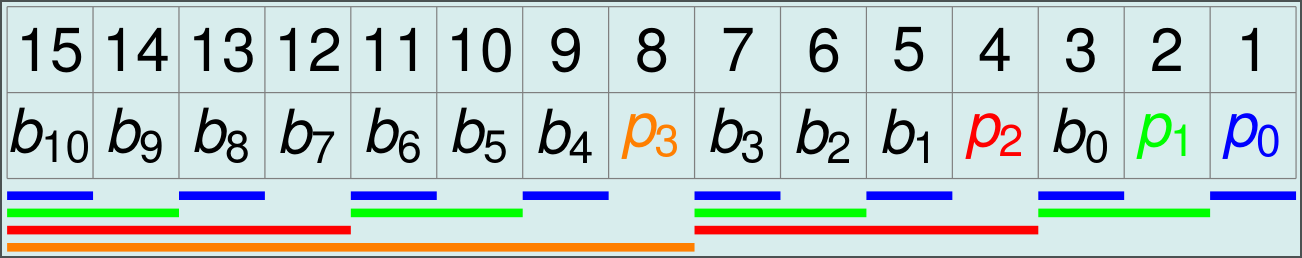
\includegraphics[width=\textwidth]{img/hammingcodes.png}
      \end{itemize}



\end{document}
